\documentclass[9pt,twocolumn,twoside]{opticajnl}
\journal{opticajournal} % use for journal or Optica Open submissions

% See template introduction for guidance on setting shortarticle option
\setboolean{shortarticle}{true}
% true = letter/tutorial
% false = research/review article

% ONLY applicable for journal submission shortarticle types:
% When \setboolean{shortarticle}{true}
% then \setboolean{memo}{true} will print "Memorandum" on title page header
% Otherwise header will remain as "Letter"
% \setboolean{memo}{true}

\usepackage{lineno}
\linenumbers % Turn off line numbering for Optica Open preprint submissions.

\title{Length-check \LaTeX\ template for preparing an article for submission to Optica Publishing Group journals AO, JOCN, JOSA A, JOSA B, OL, \emph{Optica}, \emph{Optica Quantum}, and PRJ}

\author[1,2,3]{Author One}
\author[2,*]{Author Two}
\author[1]{Author Three}

\affil[1]{Publications Department, Optica Publishing Group, 2010 Massachusetts Avenue NW, Washington DC, 20036}
\affil[2]{School of Science, University of Technology, 2000 J St. NW, Washington DC, 20036}
\affil[3]{School of Optics, University of Technology, 2000 J St. NW, Washington DC, 20036}

\affil[*]{email@my-email.com}

\begin{abstract}
This template can be used to approximate final page count for submission to Optica Publishing Group’s journals \emph{Applied Optics}, \emph{Journal of Optical Communications and Networking}, JOSA A, JOSA B, \emph{Optics Letters}, \emph{Optica}, \emph{Optica Quantum}, and \emph{Photonics Research}. Use the shortarticle/true option for \emph{Optics Letters} and short \emph{Optica} articles.  Authors may also \href{https://opticaopen.org}{submit articles} prepared using this template to the Optica Publishing Group preprint server, \href{https://preprints.opticaopen.org}{Optica Open}. However, doing so is optional. Please refer to the submission guidelines found there. You may find it helpful to use our optional \href{https://preflight.paperpal.com/partner/optica/opticapublishinggroupjournals}{Paperpal manuscript readiness check} and \href{https://languageediting.optica.org/}{language polishing service}. Note that copyright and licensing information should no longer be added to your Journal or Optica Open manuscript.
\end{abstract}

\setboolean{displaycopyright}{false} % Do not include copyright or licensing information in submission.

\begin{document}

\maketitle

\section{Introduction}
See \href{https://opg.optica.org/submit/templates/default.cfm}{Style Guide} and \href{https://opg.optica.org/submit/templates/default.cfm}{Manuscript Templates} pages for more details. 

If you have a question while using this template on {Overleaf}, please use the help menu (``?'') on the top bar to search for help or ask us a question using our \href{https://www.overleaf.com/contact}{contact form}.

\section{Corresponding author}

We require manuscripts to identify a single corresponding author. The corresponding author typically is the person who submits the manuscript and handles correspondence throughout the peer review and publication process. If other statements about author contribution and contact are needed, they can be added in addition to the corresponding author designation.

%Example with the corresponding author designated by an asterisk:

%\author{Author One\authormark{1} and Author Two\authormark{2,*}}

%\address{\authormark{1}Peer Review, Publications Department,
%Optica Publishing Group, 2010 Massachusetts Avenue NW,
%Washington, DC 20036, USA\\
%\authormark{2}Publications Department, Optica Publishing Group,
%2010 Massachusetts Avenue NW, Washington, DC 20036, USA\\
%%\authormark{3}xyz@optica.org}

%\email{\authormark{*}xyz@optica.org}}

%Example with the corresponding author designated by an asterisk and a note indicating equal contributions by two authors.

%\author{Author One\authormark{1,3} and Author %Two\authormark{2,3,*}}

%\address{\authormark{1}Peer Review, Publications Department,
%Optica Publishing Group, 2010 Massachusetts Avenue NW, %Washington, DC 20036, USA\\
%\authormark{2}Publications Department, Optica Publishing Group, %2010 Massachusetts Avenue NW, Washington, DC 20036, USA\\
%\authormark{3}The authors contributed equally to this work.\\
%\authormark{*}xyz@optica.org}}

%\section{Examples of Article Components}
%\label{sec:examples}

The sections below show examples of different article components.

\section{Figures and Tables}

Do not place figures and tables at the back of the manuscript. Figures and tables should be placed and sized as they are likely to appear in the final article. 

Figures and Tables should be labelled and referenced in the standard way using the \verb|\label{}| and \verb|\ref{}| commands.

\subsection{Sample Figure}

Figure \ref{fig:false-color} shows an example figure.

\begin{figure}[ht]
\centering
\fbox{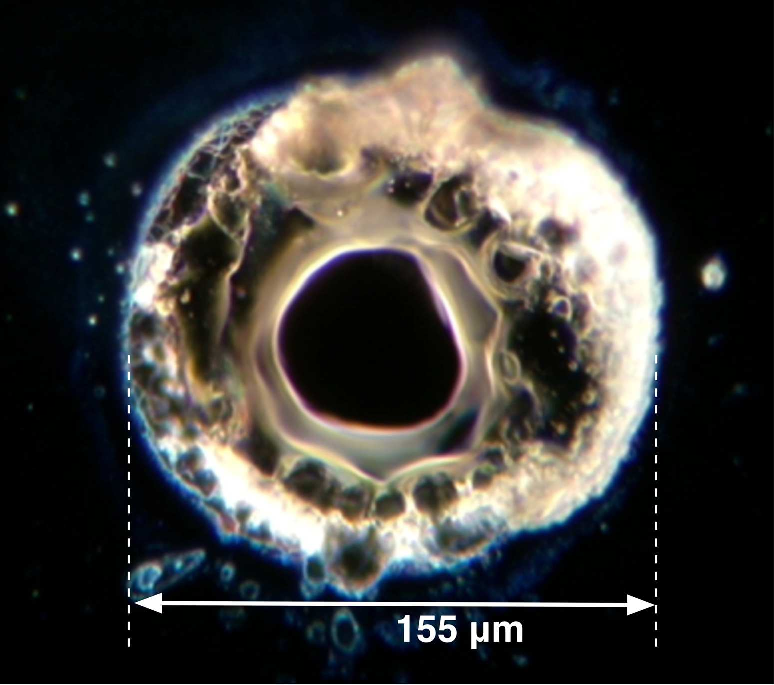
\includegraphics[width=\linewidth]{opticafig1}}
\caption{Dark-field image of a point absorber.}
\label{fig:false-color}
\end{figure}

\subsection{Sample Table}

Table \ref{tab:shape-functions} shows an example table.

\begin{table}[htbp]
\centering
\caption{\bf Shape Functions for Quadratic Line Elements}
\begin{tabular}{ccc}
\hline
local node & $\{N\}_m$ & $\{\Phi_i\}_m$ $(i=x,y,z)$ \\
\hline
$m = 1$ & $L_1(2L_1-1)$ & $\Phi_{i1}$ \\
$m = 2$ & $L_2(2L_2-1)$ & $\Phi_{i2}$ \\
$m = 3$ & $L_3=4L_1L_2$ & $\Phi_{i3}$ \\
\hline
\end{tabular}
  \label{tab:shape-functions}
\end{table}

\section{Sample Equation}

Let $X_1, X_2, \ldots, X_n$ be a sequence of independent and identically distributed random variables with $\text{E}[X_i] = \mu$ and $\text{Var}[X_i] = \sigma^2 < \infty$, and let
\begin{equation}
S_n = \frac{X_1 + X_2 + \cdots + X_n}{n}
      = \frac{1}{n}\sum_{i}^{n} X_i
\label{eq:refname1}
\end{equation}
denote their mean. Then as $n$ approaches infinity, the random variables $\sqrt{n}(S_n - \mu)$ converge in distribution to a normal $\mathcal{N}(0, \sigma^2)$.

\section{Sample Algorithm}

Algorithms can be included using the commands as shown in algorithm \ref{alg:euclid}.

\begin{algorithm}
\caption{Euclid’s algorithm}\label{alg:euclid}
\begin{algorithmic}[1]
\Procedure{Euclid}{$a,b$}\Comment{The g.c.d. of a and b}
\State $r\gets a\bmod b$
\While{$r\not=0$}\Comment{We have the answer if r is 0}
\State $a\gets b$
\State $b\gets r$
\State $r\gets a\bmod b$
\EndWhile\label{euclidendwhile}
\State \textbf{return} $b$\Comment{The gcd is b}
\EndProcedure
\end{algorithmic}
\end{algorithm}

\subsection{Supplementary materials in Optica Publishing Group journals}
Optica Publishing Group journals allow authors to include supplementary materials as integral parts of a manuscript. Such materials are subject to peer-review procedures along with the rest of the paper and should be uploaded and described using the Prism manuscript system. Please refer to the \href{https://opg.optica.org/submit/style/supplementary_materials.cfm}{Author Guidelines for Supplementary Materials in Optica Publishing Group Journals} for more detailed instructions on labeling supplementary materials and your manuscript. For preprints submitted to Optica Open a link to supplemental material should be included in the submission, but do not upload the material.

\textbf{Authors may also include Supplemental Documents} (PDF documents with expanded descriptions or methods) with the primary manuscript. At this time, supplemental PDF files are not accepted for JOCN or PRJ. To reference the supplementary document, the statement ``See Supplement 1 for supporting content.'' should appear at the bottom of the manuscript (above the References heading). Supplemental documents are not accepted for Optica Open preprints.

\begin{figure}[ht!]
\centering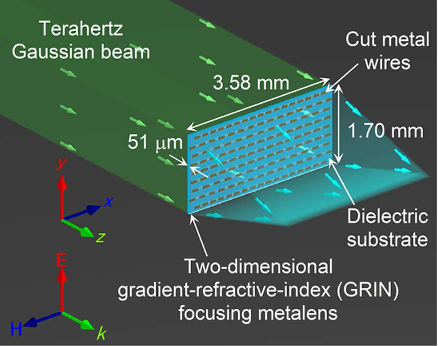
\includegraphics{opticafig2}
\caption{Terahertz focusing metalens.}
\end{figure}


\subsection{Sample Dataset Citation}

1. M. Partridge, "Spectra evolution during coating," figshare (2014), http://dx.doi.org/10.6084/m9.figshare.1004612.

\subsection{Sample Code Citation}

2. C. Rivers, "Epipy: Python tools for epidemiology," Figshare (2014) [retrieved 13 May 2015], http://dx.doi.org/10.6084/m9.figshare.1005064.

\section{Backmatter}
Backmatter sections should be listed in the order Funding/Acknowledgment/Disclosures/Data Availability Statement/Supplemental Document section. An example of backmatter with each of these sections included is shown below.

\begin{backmatter}
\bmsection{Funding} Content in the funding section will be generated entirely from details submitted to Prism. Authors may add placeholder text in the manuscript to assess length, but any text added to this section in the manuscript will be replaced during production and will display official funder names along with any grant numbers provided. If additional details about a funder are required, they may be added to the Acknowledgments, even if this duplicates information in the funding section. See the example below in Acknowledgements. For preprint submissions, please include funder names and grant numbers in the manuscript.

\bmsection{Acknowledgments} The section title should not follow the numbering scheme of the body of the paper. Additional information crediting individuals who contributed to the work being reported, clarifying who received funding from a particular source, or other information that does not fit the criteria for the funding block may also be included; for example, ``K. Flockhart thanks the National Science Foundation for help identifying collaborators for this work.''

\bmsection{Disclosures} Disclosures should be listed in a separate section at the end of the manuscript. List the Disclosures codes identified on the \href{https://opg.optica.org/submit/review/conflicts-interest-policy.cfm}{Conflict of Interest policy page}. If there are no disclosures, then list ``The authors declare no conflicts of interest.''

\smallskip

\noindent Here are examples of disclosures:


\bmsection{Disclosures} ABC: 123 Corporation (I,E,P), DEF: 456 Corporation (R,S). GHI: 789 Corporation (C).

\bmsection{Disclosures} The authors declare no conflicts of interest.


\bmsection{Data Availability Statement} A Data Availability Statement (DAS) will be required for all submissions beginning 1 March 2021. The DAS should be an unnumbered separate section titled ``Data Availability'' that
immediately follows the Disclosures section. See the \href{https://opg.optica.org/submit/review/data-availability-policy.cfm}{Data Availability Statement policy page} for more information.

There are four common (sometimes overlapping) situations that authors should use as guidance. These are provided as minimal models, and authors should feel free to
include any additional details that may be relevant.



\begin{enumerate}
\item When datasets are included as integral supplementary material in the paper, they must be declared (e.g., as "Dataset 1" following our current supplementary materials policy) and cited in the DAS, and should appear in the references.

\bmsection{Data availability} Data underlying the results presented in this paper are available in Dataset 1, Ref. [3].

\item When datasets are cited but not submitted as integral supplementary material, they must be cited in the DAS and should appear in the references.

\bmsection{Data availability} Data underlying the results presented in this paper are available in Ref. [3].

\item If the data generated or analyzed as part of the research are not publicly available, that should be stated. Authors are encouraged to explain why (e.g.~the data may be restricted for privacy reasons), and how the data might be obtained or accessed in the future.

\bmsection{Data availability} Data underlying the results presented in this paper are not publicly available at this time but may be obtained from the authors upon reasonable request.

\item If no data were generated or analyzed in the presented research, that should be stated.

\bmsection{Data availability} No data were generated or analyzed in the presented research.
\end{enumerate}

\bigskip

\noindent Data availability statements are not required for preprint submissions.

\bmsection{Supplemental document}
See Supplement 1 for supporting content. 

\end{backmatter}

\section{References}

Note that \emph{Optics Letters} and \emph{Optica} short articles use an abbreviated reference style. Citations to journal articles should omit the article title and final page number; this abbreviated reference style is produced automatically when the \emph{Optics Letters} journal option is selected in the template, if you are using a .bib file for your references.

\bigskip
\noindent Add citations manually or use BibTeX. See \cite{Zhang:14,OPTICA,FORSTER2007,testthesis,manga_rao_single_2007}. List up to three author names in references, and if there are more than three authors use \emph{et al.} after that.

% Bibliography
\bibliography{sample}

% Full bibliography added automatically for Optics Letters submissions; the following line will simply be ignored if submitting to other journals.
% Note that this extra page will not count against page length
\bibliographyfullrefs{sample}

%Manual citation list
%\begin{thebibliography}{1}
%\bibitem{Zhang:14}
%Y.~Zhang, S.~Qiao, L.~Sun, Q.~W. Shi, W.~Huang, %L.~Li, and Z.~Yang,
 % \enquote{Photoinduced active terahertz metamaterials with nanostructured
  %vanadium dioxide film deposited by sol-gel method,} Opt. Express \textbf{22},
  %11070--11078 (2014).
%\end{thebibliography}

% Please include bios and photos of all authors for aop articles
\ifthenelse{\equal{\journalref}{aop}}{%
\section*{Author Biographies}
\begingroup
\setlength\intextsep{0pt}
\begin{minipage}[t][6.3cm][t]{1.0\textwidth} % Adjust height [6.3cm] as required for separation of bio photos.
  \begin{wrapfigure}{L}{0.25\textwidth}
    \includegraphics[width=0.25\textwidth]{john_smith.eps}
  \end{wrapfigure}
  \noindent
  {\bfseries John Smith} received his BSc (Mathematics) in 2000 from The University of Maryland. His research interests include lasers and optics.
\end{minipage}
\begin{minipage}{1.0\textwidth}
  \begin{wrapfigure}{L}{0.25\textwidth}
    \includegraphics[width=0.25\textwidth]{alice_smith.eps}
  \end{wrapfigure}
  \noindent
  {\bfseries Alice Smith} also received her BSc (Mathematics) in 2000 from The University of Maryland. Her research interests also include lasers and optics.
\end{minipage}
\endgroup
}{}


\end{document}
